\section{Ergebnisse} % (fold)
    \label{sec:ergebnisse}
    \begin{figure}[h]
        \centering
        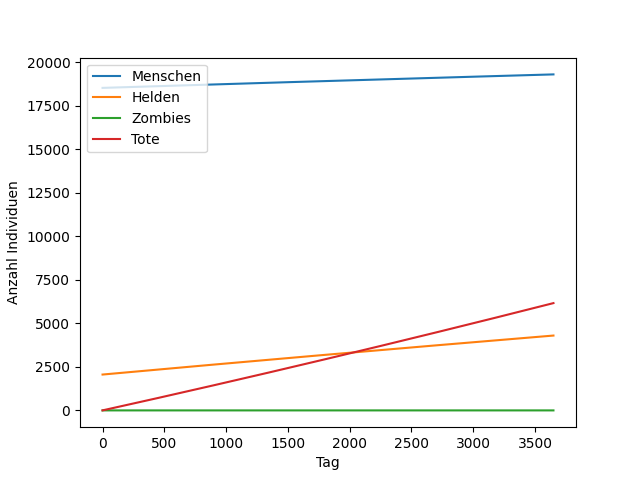
\includegraphics[width=1\textwidth]{normal.png}
        \caption{Die Simulation ohne Parasit}
        \label{fig:normal}
    \end{figure}
    \autoref{fig:normal} simuliert die Bevölkerungsentwicklung unter normalen Umständen, also ohne den Parasit. Die initiale Anzahl Menschen beträgt 18537,3 und die der Helden etwa 2059,7. Es zeichnet sich über die 10 beobachteten Jahre ein klarer Anstieg ab.
    \newpage
    \begin{figure}[h]
        \centering
        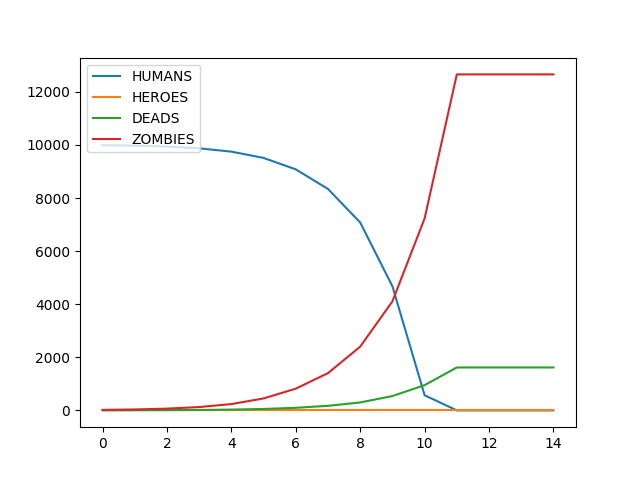
\includegraphics[width=1\textwidth]{zombified_no_heroes.png}
        \caption{Die Simulation ohne Helden}
        \label{fig:no_heroes}
    \end{figure}
    \autoref{fig:no_heroes} stellt den Verlauf der Pandemie dar, wenn es keine Individuen der Helden-Spezies gäbe. Es beginnt mit 20597 Menschen und einem Zombie. Nach 10 Tagen kündigt sich die Apokalypse an. Die Anzahl an Zombies und Toten steigt exponentiell an, während die Menschen dementsprechend in großer Zahl weniger werden. Die Zombies besetzen letztendlich nach 20 Tagen die Stadt mit einer Schar von über 12000 Infizierten.
    \newpage
    \begin{figure}[h]
        \centering
        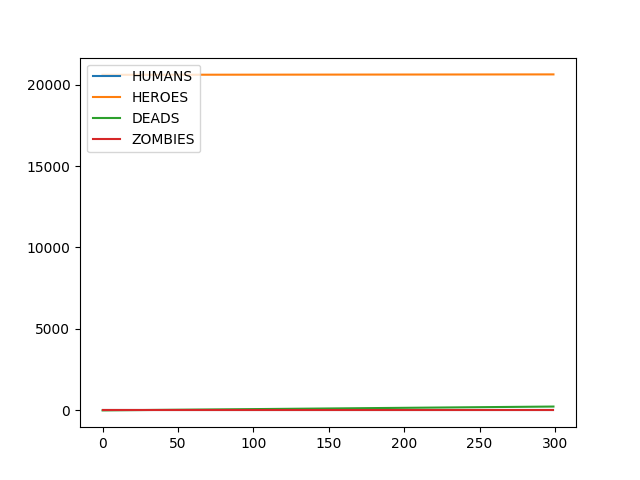
\includegraphics[width=1\textwidth]{zombified_all_heroes.png}
        \caption{Die Simulation ohne Menschen}
        \label{fig:no_humans}
    \end{figure}
    \autoref{fig:no_humans} zeigt den Einfluss der Helden auf die Zombies. Es gibt am Anfang 20597 Helden und 2000 Zombies. Nach 20 Tagen sind alle Helden tot und die Zombies um einen Bruchteil in ihrer Anzahl verringert worden.
    \newpage
    \begin{figure}[h]
        \centering
        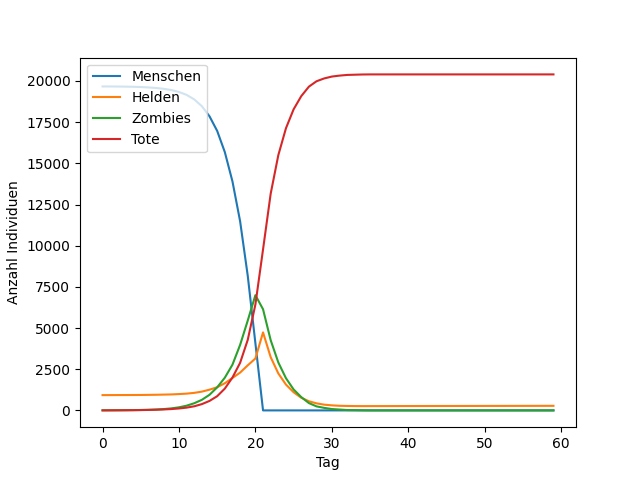
\includegraphics[width=1\textwidth]{zombified.png}
        \caption{Die Simulation mit allen Spezies vetreten}
        \label{fig:simulation}
    \end{figure}
    \autoref{fig:simulation} visualisiert den Verlauf der gesamten modellierten Simulation. Es gibt initial 18537,3 Menschen und 2059,7 Helden, ein Zombie ist in der Stadt. Wie in \autoref{fig:no_heroes} gibt es nach 20 Tagen keine Menschen mehr, aber davon sind etwa 1300 zu Helden geworden. Dies bildet einen Wendepunkt, da nun Helden und Zombies dezimiert und die Zombies besiegt werden.
% section ergebnisse (end)
